\section{Design} \label{sec:base}

A complete design---a design that detects misbehavior by both CAs and CT logs
within our strong threat model---necessitates a considerable degree of
complexity. In this section, we present such a full design by breaking it up
into four phases as shown in Figure~\ref{fig:design}, demonstrating the need for
the complexity in each step. Later, Section~\ref{sec:incremental} presents two
incremental versions of the full design that are less complicated but at the
cost of either only achieving a weaker security goal or by having a weaker
threat model.

A simple design is one that only validates SCTs, which is how CT in Google
Chrome and other browsers is currently deployed. However, such a design does not
stand up against a malicious CA and logs working in concert; auditing is needed.

\begin{figure*}
    \centering
	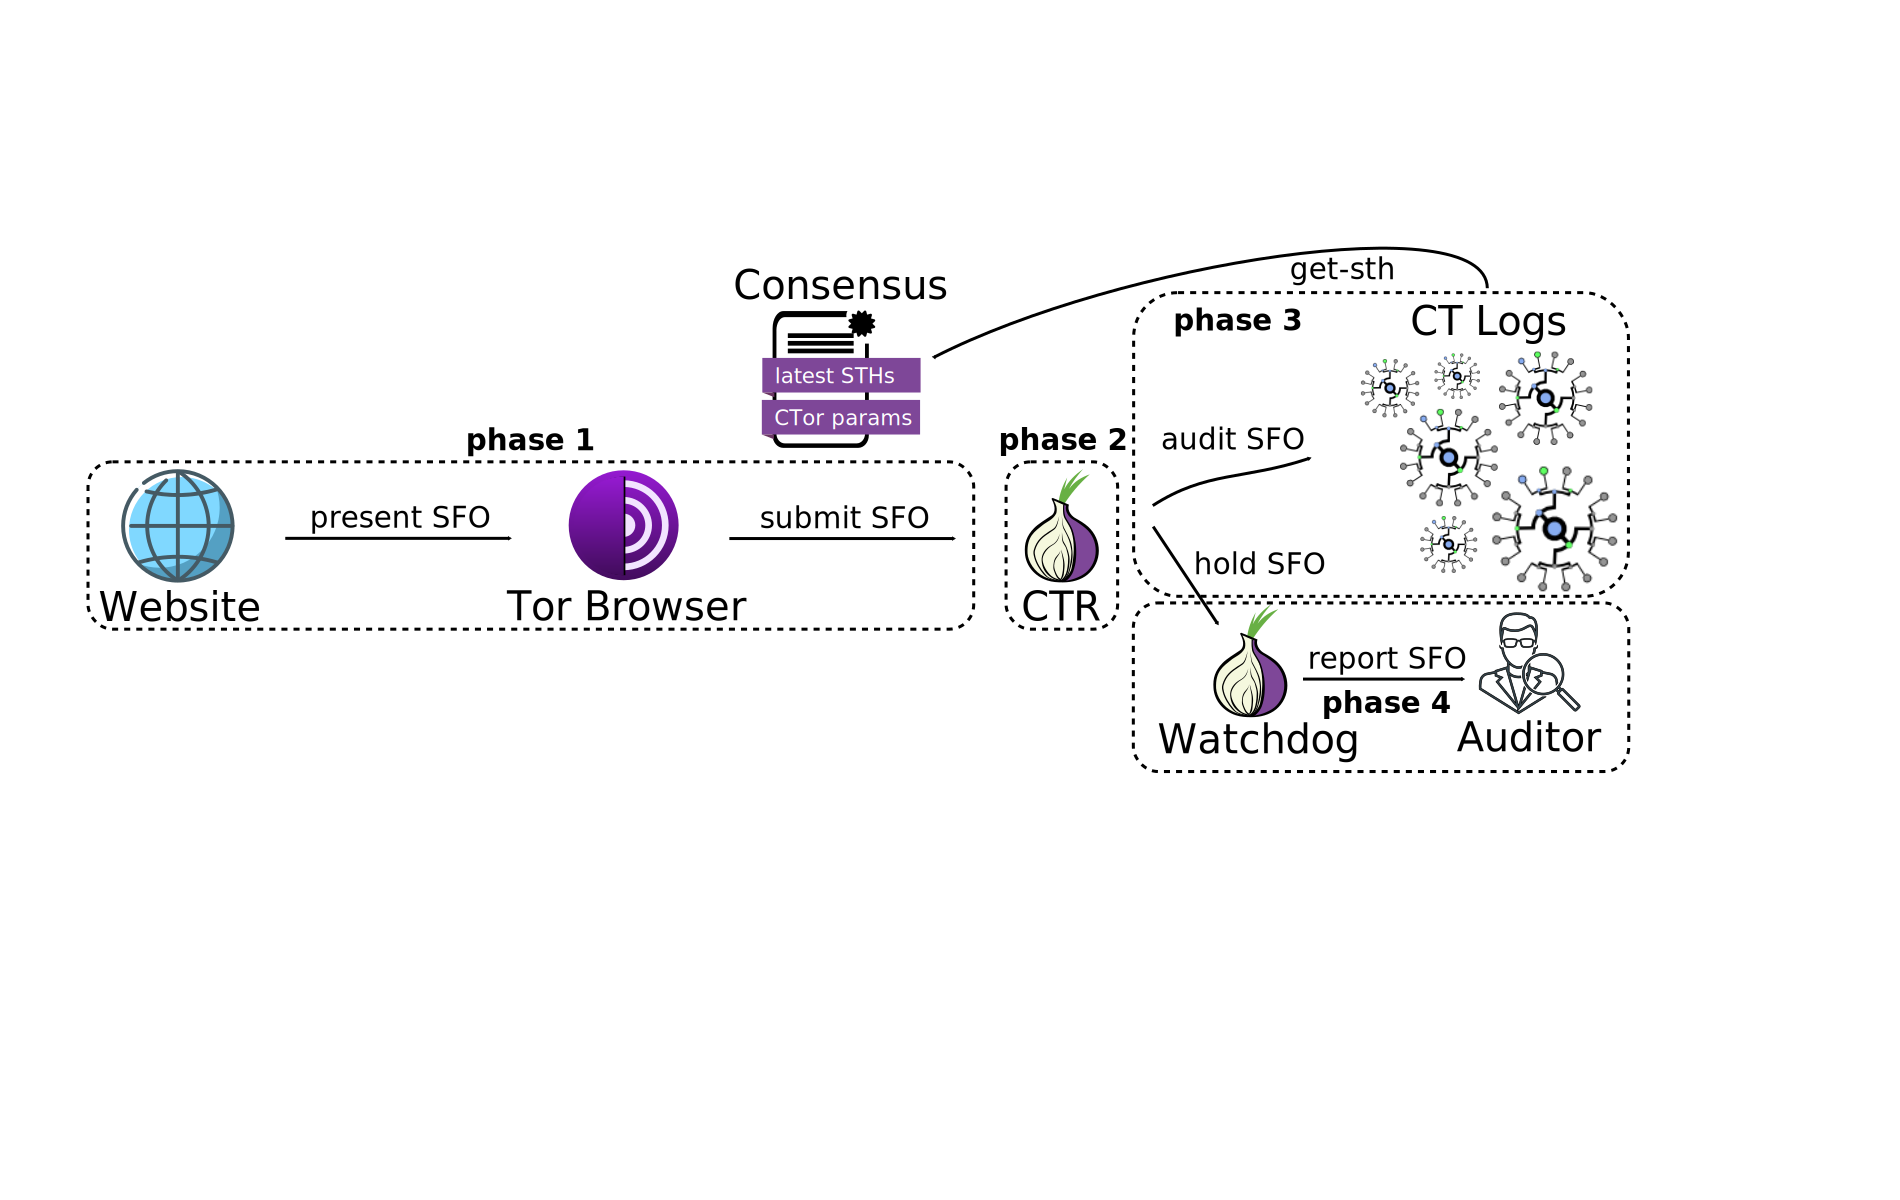
\includegraphics[width=0.8\textwidth]{img/design}
	\vspace{-8px}
	\caption{%
		An overview of the four phases of the full CTor design. In phase 1 Tor
	Browser submits a SFO (SCT Feedback Object) to a Certificate Transparency
	Relay (CTR), followed by phase 2 where the CTR buffers the SFO. In phase 3
	the relays attempts to audit the SFO, and in case of failure, it reports the
	SFO to an auditor with the help of a watchdog CTR in phase 4.}
	\label{fig:design}
	\vspace{-10px}
\end{figure*}

\subsection{Phase~1---Tor Browser} \label{sec:base:phase1}

The least complicated auditing design would be one where Tor Browser receives a
TLS Certificate and accompanying SCTs (we will refer to this bundle as an SCT
Feedback Object or SFO) and talks to the corresponding logs, over Tor,
requesting an inclusion proof for the SCT. In an ordinary browser, this would be
an unacceptable leak to the log of browsing behavior associated with an IP
address; performing this request over Tor leaks real-time browsing behavior but
not the user's IP address.

An immediate problem with this design is that a primary requirement of Tor
Browser is to persist no data about browsing behavior after the application
exits. If we assume a user's browser is not left open for long periods of time,
the inclusion proof request can be easily circumvented by the attacker by
supplying a fresh SCT whose MMD has not completed---thus no inclusion proof can
be provided as per the CT standard. A second problem is that the STH returned
from any inclusion proof exists in a trust vacuum---there is no way to know that
it is consistent with other STHs and not part of a split view.

The evolved proposal adds two components: a list of STHs that the browser will
receive over a trusted channel and the participation of a third party with the
ability to persist data and perform auditing actions at a later time.

A single third party used by all Tor Browser users would receive a considerable
aggregation of browsing behavior and would need to scale in-line with the entire
Tor network. A small number of auditors presents privacy and
single-point-of-failure concerns. A large number would be ideal but presents
difficulties in curation and independent management and still requires scaling
independent of the Tor network. These concerns do not entirely preclude the
design, but they can be easily avoided by reusing relays in the Tor Network as
our trusted third parties: we call the relays so designated Certificate
Transparency Relays (CTR).

Now, when the browser is completing the TLS handshake they simultaneously either
pass the SFO to a CTR (if the MMD of the SCT has not elapsed) or query the log
themselves asking for an inclusion proof to a trusted STH\@.  However, if we
presume the attacker can serve an exploit to the browser, the latter behavior is
immediately vulnerable. The log, upon receiving an inclusion proof fetch for an
SCT that it knows is malicious, will delay responding. The TLS connection in the
browser, having succeeded, will progress to the HTTP request and response, at
which point the exploit will be served, and the SFO (containing the
cryptographic evidence of CA and log misbehavior) will be deleted by the exploit
code. While blocking the TLS connection until the CT log responds is an option,
experience related to OCSP hard-fail indicates that this notion is doomed to
fail~\cite{no-hard-fail}.

The third evolution of our proposal has the Browser submit the SFO to the CTR
immediately upon receipt in all cases. A consequence of this shift is that the
trusted STH list no longer needs to be delivered to the browser but rather the
CTRs. To mitigate the risk of an exploit finding the CTR and disclosing its
identity to the attacker (who could then target it for Denial of Service), we
prepare CTR circuits ahead of time and close and discard them as soon as the SFO
is sent, allowing the SFO submission to race with the TLS connection completion
and HTTP request/response.  An added detail is to block the TLS connection in
the situation that an SFO is unusually large, as defined by a parameter
\texttt{ct-large-sfo-size}. A large SFO may indicate an attempt to win that race
between SFO submission and exploitation, and the parameter can be chosen such
that it happens extremely rarely on legitimate connections.

The third evolution of our proposal exhibits all the protections we can
reasonably achieve within the browser. We summarize this phase with the
following algorithm that provides more explicit steps and details, and add a
parameter \texttt{ct-submit-pr} that indicates a probability that an SFO is
submitted to a CTR---this provides probabilistic security while providing the
ability to adjust submission rates to account for CTR scaling issues. Given an
incoming SFO $s$, we follow the below steps: % The bit introducing
\texttt{ct-submit-pr} can be better.

\begin{enumerate}
    \item Raise a certificate error and stop if the certificate chain of $s$
        is not rooted in TB's trust store.
    \item Raise a certificate transparency error and stop if the SCTs of $s$
        fail TB's CT policy.
    \item If $\mathsf{len}(s) < \texttt{ct-large-sfo-size}$, accept $s$ and
        conduct the remaining steps in the background while the TLS connection
        and HTTP request/response proceed. If $\mathsf{len}(s) \geq
        \texttt{ct-large-sfo-size}$ pause the TLS handshake, complete the
        remaining steps and then accept~$s$ as valid and continue the handshake
        and HTTP request/response.
    \item Flip a biased coin based on \texttt{ct-submit-pr} and stop if the
        outcome indicates no further auditing.
    \item Submit $s$ to a random CTR's SFO-endpoint on a pre-built circuit.
        The circuit used for submission is closed immediately after use without
        waiting for any acknowledgment.
\end{enumerate}

\subsection{Phase 2---Buffering} \label{sec:base:phase2}

Once received, the most straightforward thing for a CTR to do is to contact the
issuing log and request an inclusion proof relative to a trusted STH\@. (And if
the SCT's MMD has not elapsed, hold the SFO until it has.) However, this
proposal has two flaws, the first of which leads us to the design of Phase 2.

Immediately contacting the log about an SFO (a) allows the log to predict when
exactly it will receive a request about an SFO and (b) discloses real-time
browsing behavior to the log. The former problem means that an attacker can
position resources for perpetuating an attack ahead-of-time, as well as letting
it know with certainty whether a connection was audited (based on
\texttt{ct-submit-pr}). The latter is some amount of information leakage that
can help with real-time traffic analysis. 

Because a CTR must support storing SCTs regardless, we can schedule an event in
the future for when each SFO would be sent. Adding a per-SFO value sampled from
\texttt{ct-delay-dist} effectively adds stop-and-go
mixing~\cite{kesdogan:ih1998} to the privacy protection, but where there is only
one mix (CTR) between sender (client) and receiver (CT log). So there is no
point in a client-specified interval-start-time such that the mix drops messages
arriving before then, and there is no additional risk in having the interval end
time set by the mix rather than the sender. This means both that some SFOs a
client sends to a CTR at roughly the same time might be in different batches of
SFOs sent to a CT log and that SFOs submitted to that CTR by other honest
clients are more likely to be mixed with these.


In addition to storing SFOs for mixing effects, we also add a layer of caching
to alleviate stored data {\bf \color{red} Does ``to alleviate stored data'' just
mean ``to reduce the overhead of storing data''?}\\
and unnecessary log connections and data disclosure. So with
regards to some CT circuit, an incoming SFO $s$ is processed as follows:
\begin{enumerate}
    \item\label{enm:storage:close} Close the current circuit to enforce one-time
        usage.
    \item\label{enm:storage:unrecognized} Discard all SCTs in the SFO for logs the
        CTR is not aware of; if no SCTs remain then discard the entire SFO\@.
    \item\label{enm:storage:cached}
        Stop if $s$ is cached (see Section~\ref{sec:base:phase3}) or already
        pending to be audited.
    \item\label{enm:storage:fix-log} Sample a CT log $l$ that issued a
        remaining SCT in~$s$.
    \item\label{enm:storage:audit-after} Compute an \texttt{audit\_after}
		time~$t$, see Figure~\ref{fig:audit-after}.
    \item\label{enm:storage:store} Add $(l,t,s)$ to a buffer of pending SCTs to audit.
\end{enumerate}

Recall from Section~\ref{sec:background:ct} that an inclusion proof is fetched
with regards to an STH\@.  As such, we discard SCTs that cannot be verified due
to lack of a trusted STH\@.  The sampled CT log $l$ now refers to an entity that
issued an SCT in the submitted SFO, and it will be challenged to prove inclusion
in phase~3 sometime after the \texttt{audit\_after} timestamp $t$ elapsed. We
can choose one SCT (and therefore log) at random from the SFO, because it is
sufficient to catch only one misbehaving log so long as we report the entire
SFO, allowing for other malicious logs to be identified. (And if one log is
malicious and others are honest; the honest logs will have ensured publication
of the malicious certificate.)


The \texttt{audit\_after} timestamp specifies the earliest point in time that an
SCT from an SFO will be audited in Phase~3, which adds random noise that
obfuscates real-time browsing patterns in the Tor network and complicates
predictions of when it is safe to assume no audit will take place.  If memory
becomes a scarce resource, pending triplets should be deleted at
random~\cite{nordberg}. Figure~\ref{fig:audit-after} shows that $t$ takes the
log's MMD into account.  This is one of two parts that prevent \emph{early
signals} to the issuing CT logs that an SFO is being audited.  For example, if
an SFO is audited before the MMD elapsed, the issuing CT log could simply merge
the underlying certificate chain to avoid any MMD violation.

% TODO: If we're going to say 'one of two early signals' we need to clearly identify the other one. And it's not clear to me what else specifically is considered such an early signal.

\begin{figure}
	\centering
	\pseudocode[linenumbering, syntaxhighlight=auto]{%
		\textrm{t} \gets \mathsf{now}() +
			\mathsf{MMD} +
			\mathsf{random}(\texttt{ct-delay-dist}) \\
		\pcif \textrm{SCT.timestamp} + \textrm{MMD} <
				\mathsf{now}():\\
			\pcind\textrm{t} \gets \mathsf{now}() +
				\mathsf{random}(\texttt{ct-delay-dist})
	}
	\caption{%
		Algorithm that computes an \texttt{audit\_after} timestamp $t$.
	}
	\label{fig:audit-after}
\end{figure}

\subsection{Phase 3---Auditing} \label{sec:base:phase3}

As alluded to in Phase 2, there is a second problem why the simple behavior of
`contact the log and request an inclusion proof' is unacceptable. We include the
ability to DoS an individual Tor relay in our threat model---if the log knows
which CTR holds the evidence of its misbehavior, it can take the CTR offline,
wiping the evidence of the log's misbehavior from its memory. 

We can address this concern in a few ways. The simple proposal of contacting the
log over a Tor circuit will not suffice---a log can tag each CTR by submitting
unique SFOs to them all, and recognize the CTR when they are submitted. Even
using a unique Tor circuit for each SFO might not suffice to prevent effective
tagging attacks. For example, after tagging all CTRs, a malicious log could
ignore all but innocuous untagged requests and tagged requests matching tags for
whichever CTR it responds to first. If exponential backoff is supported, the
rest of the CTRs will backoff repeated attempts to fetch a proof until the first
CTR has emptied itself of pending SFOs. Then the log can repeat this process
until it receives the offending SFO\@. With high probability this will come in
the midst of a string circuits with tags from a particular CTR (as opposed to
being requested on the first circuit from some CTR). This might result in many
CTRs reporting the log as inaccessible for days, but that is not the same as
direct evidence of misbehavior.

{\bf \color{red} Paul did not understand this
  despite-one-SFO-per-circuit tagging attack as it was written and had
  to write it up differently till he did. I think I've captured the
  attack, which is the most important thing. Let me know.\\ \\
  I still don't see how this is likely to be effective given (a) how long it
  will take CTRs to send all their currently pending SFOs, (b) that the log
  won't be able to tell when a given CTR has finished sending all the SFOs it
  has pending for that log, so OK to move to the next one, (c) the expected
  number of CTRs to run through till the offending SFO pops up (if ever
  depending on coin flips), and (d) with the randomized delay, there is a fair
  chance that the offending SFO won't come up the first time a CTR is the
  current target.\\ \\
  Totally making numbers up: if there are 25 CTRs in the network, and
  it takes an hour to be reasonably sure the current target has run
  through its whole current pending pile, and expected iterations till
  an offending SFO comes up is 2, then many CTRs will have noticed
  the log as unavailable for days. I guess this is a much lesser
  offense and tried to note it, though on top of everything else
  it would seem to make likely that the attack can't be conducted
  more than once or twice since being repeatedly unavailable broadly
  might be an issue.}


While there are ways to detect this attack after-the-fact, and there may be ways
to mitigate it, a more robust design would tolerate the disclosure of a CTRs
identity to the log without allowing a Denial-of-Service attack to erase
evidence of misbehavior.  The simple approach is to write the data to disk prior
to contacting the log; however, Tor relays are explicitly designed not to write
data about user behavior to disk unless debug-level logging is enabled. Relay
operators have expressed an explicit desire to never have any user data
persisted to disk, as it changes the risk profile of their servers with regards
to search, seizure, and forensic analysis.

The evolved design is to have the CTR work with a partner CTR---we call it a
watchdog---whom they choose at random and contact over a Tor circuit. Prior to
talking to a log, the CTR provides the watchdog with the SFO it is about to
submit. After an appropriate response from the log, the CTR tells the watchdog
that SFO has been adequately addressed.

Each CTR maintains a single shared circuit that is used to interact with all CT
logs known to the CTR\@. (We are not using one circuit per SFO given the
overhead and the unclear security benefit noted above.) For \emph{each} such CT
log $l$, the CTR runs the following steps indefinitely:
\begin{enumerate}
    \item\label{enm:auditing:backoff} Sample a delay $d \gets
        \mathsf{random}(\texttt{ct-backoff-dist})$ and wait until $d$ time units
        elapsed.
    \item Connect to a random watchdog CTR\@.
    \item\label{enm:auditing:loop} For each pending buffer entry $(l',s,t)$,
    where $l' = l$ and $t <= \mathsf{now}()$:
		\begin{enumerate}
			\item\label{enm:ext:auditing:watchdog} Share $s$ with the current
				watchdog.
			\item\label{enm:ext:auditing:challenge} Challenge the log to prove
                                  inclusion to a known STH, waiting for
                                  \texttt{ct-log-timeout} before timing out.
				\begin{itemize}
					\item\label{enm:ext:auditing:challenge:success} On valid
						proof: send an acknowledgment to the watchdog, then
						cache $s$ and discard it.
					\item\label{enm:ext:auditing:challenge:fail} On any other
						outcome: discard $s$, close circuit to the watchdog CTR,
						and go to step~1.
				\end{itemize}
		\end{enumerate}
\end{enumerate}

\subsection{Phase 4---Reporting}

At any given time, a CTR may be requesting inclusion proofs from logs (we will
refer to this role as the log-challenger) and may also be a watchdog for one or
more other CTRs. A CTR acting as a watchdog will have at most one SFO held
temporarily for each log-challenger it is interacting with. If a response from
the log-challenger is not received within \texttt{ct-watchdog-timeout}, it
becomes the watchdog's responsibility to raise it for human intervention. This
end-stage process that begins with the watchdog's receipt of a suspicious SFO
and culminates in human review is referred to as auditing, and left
mostly-unspecified.

Because human review and publication\footnote{Most likely on the ct-policy group
at \url{https://groups.google.com/a/chromium.org/forum/\#!forum/ct-policy}} is
critical, we envision that the watchdog (which is a Tor relay that may not be
closely monitored) provides the SFO to an independent auditor run by a human
closely monitoring its operation. When arriving at the design of the CTR being a
role played by a Tor relay, we eschewed separate auditors because of the lack of
automatic scaling with the Tor network, the considerable aggregation of browsing
behavior across the Tor network, and the difficulties of curation and validation
of trustworthy individuals. SFOs submitted to auditors at this stage have been
filtered through the CTR layer, resulting in an exponentially smaller load (and
data exposure) for auditors and allowing a smaller number of them to operate
without needing to scale with the network.

While we consider all auditors trusted---the watchdog needs to take precautions
talking to them because the network is not trusted\footnote{While our threat
model, and Tor's, precludes a global network adversary, we both include partial
network control within the threat model.}. If the watchdog contacted the auditor
without a Tor circuit, an adversary watching the auditors' network connections
could induce a watchdog to contact the auditor, learn the watchdog's identity,
pause their network connection, and perform a Denial of Service attack erasing
the evidence of misbehavior. To mitigate this, the watchdog can contact an
auditor as soon as it receives an SFO it should report; however it must contact
the auditor over a Tor circuit. If a successful acknowledgement from the auditor
is not received within \texttt{ct-auditor-timeout}, the SFO is buffered and
should be re-presented to the same auditor after a random delay.

When an auditor receives an SFO, it should persist it to durable storage until
it can be successfully resolved to a trusted STH\@. Once so persisted, the
auditor can begin querying the log itself asking for an inclusion proof. If no
inclusion proof can be provided after some threshold of time, or the inclusion
proof shows evidence of a MMD violation, the auditor software should raise the
details to a human operator for investigation.

Separately, the auditor should be retrieving the current Tor consensus and
ensuring that a consistency proof can be provided between STHs from the older
consensus and the newer. If consistency can be established, the older STH can be
discarded. If consistency cannot be established after some threshold of time,
the auditor software should raise the details to a human operator for
investigation. It would also be possible for an auditor to monitor a log's
uptime and report on excessive downtime.

\subsection{Additional Details} \label{sec:base:consensus}

\subsubsection{CTR Flag} \label{sec:base:consensus:ctr-flag} Within the Tor
consensus, the existing \texttt{known-flags} item determines the different flags
that the consensus might contain.  We add another flag named \texttt{CTR}, which
indicates that a Tor relay should support CT-auditing as described here. For
now, assume that a relay qualifies as a CTR if it is flagged as \texttt{stable}
and not \texttt{exit}, to spare the relatively sparse exit bandwidth and only
use relays that can be expected to stay online. Section~\ref{sec:privacy}
discusses trade-offs in the assignment of the \texttt{CTR} flag.

\subsubsection{Trusted STHs}
Tor's consensus should capture a fixed view of the CT landscape by publishing
STHs from all recognized logs.  A CT log is recognized if a majority of
directory authorities proposed a \texttt{ct-log-info} item, which contains a
log's ID, public key, base URL, MMD, and most recent STH\@.  Each directory
authority proposes its own STH, and agrees to use the most recent STH as
determined by timestamp and lexicographical order.  Since CTRs verify inclusion
with regards to SCTs that TB accepts, the CT logs recognized by TB must be in
Tor's consensus.

\subsubsection{Trusted Auditors}
Tor's directory authorities also majority-vote on \texttt{ct-auditor} items,
which pin base URLs and public keys of CT auditors that watchdogs contact in
case that any log misbehavior is suspected.  A watchdog triggers if the time
specified by \texttt{ct-watchdog-timeout} elapses without receiving any
acknowledgment.  The following auditor submission is governed by a
\texttt{ct-auditor-timeout}, which, if triggered, results in a resubmission
later on.

\subsubsection{Other Parameters} \label{sec:base:consensus:params} Directory
authorities influence the way in which TB and CTRs behave by voting on other
necessary parameters. Below, the value of an item is computed as the median of
all votes.
\begin{description}
    \item[ct-submit-pr:] A floating-point in $[0,1]$ that determines Tor
        Browser's submission probability.  For example, $0$ disables submissions
        while $0.10$ means that every 10$^{\mathsf{th}}$ SFO is sent to a random
        CTR on average.
    \item[ct-large-sfo-size:] A natural number that determines how many
        wire-bytes a normal SFO should not exceed.  As outlined in
        Section~\ref{sec:base:phase1}, excessively large SFOs are subject to
        stricter verification criteria.
    \item[ct-log-timeout:] A natural number that determines how long a CTR waits
        before concluding that a CT log is unresponsive, e.g., 10~seconds. As
        outlined in Section~\ref{sec:base:phase3}, timeouts trigger implicit
        resubmissions.
    \item[ct-delay-dist:] A distribution that determines how long a CTR should
        wait at minimum before auditing a submitted SFO\@.  As outlined in
        Section~\ref{sec:base:phase2}, random noise is added, e.g., on the order
        of minutes to an hour.
    \item[ct-backoff-dist:]
        A distribution that determines how long a CTR should wait between two
        auditing instances, e.g., a few minutes on average.  As outlined in
        Section~\ref{sec:base:phase3}, CTRs audit pending SFOs in batches at
        random time intervals to spread out log overhead.
    \item[ct-watchdog-timeout]
    \item[ct-auditor-timeout]
\end{description}
